%% LORENZO
%7. Merchant dashboard. Where the merchant can:
%    a. Add, refill and remove products
%    b. Update products description
%    c. Have an overview of all the orders that has been created on the application
\UC{Aggiunta Prodotto}
\begin{figure}[H]
    \centering
    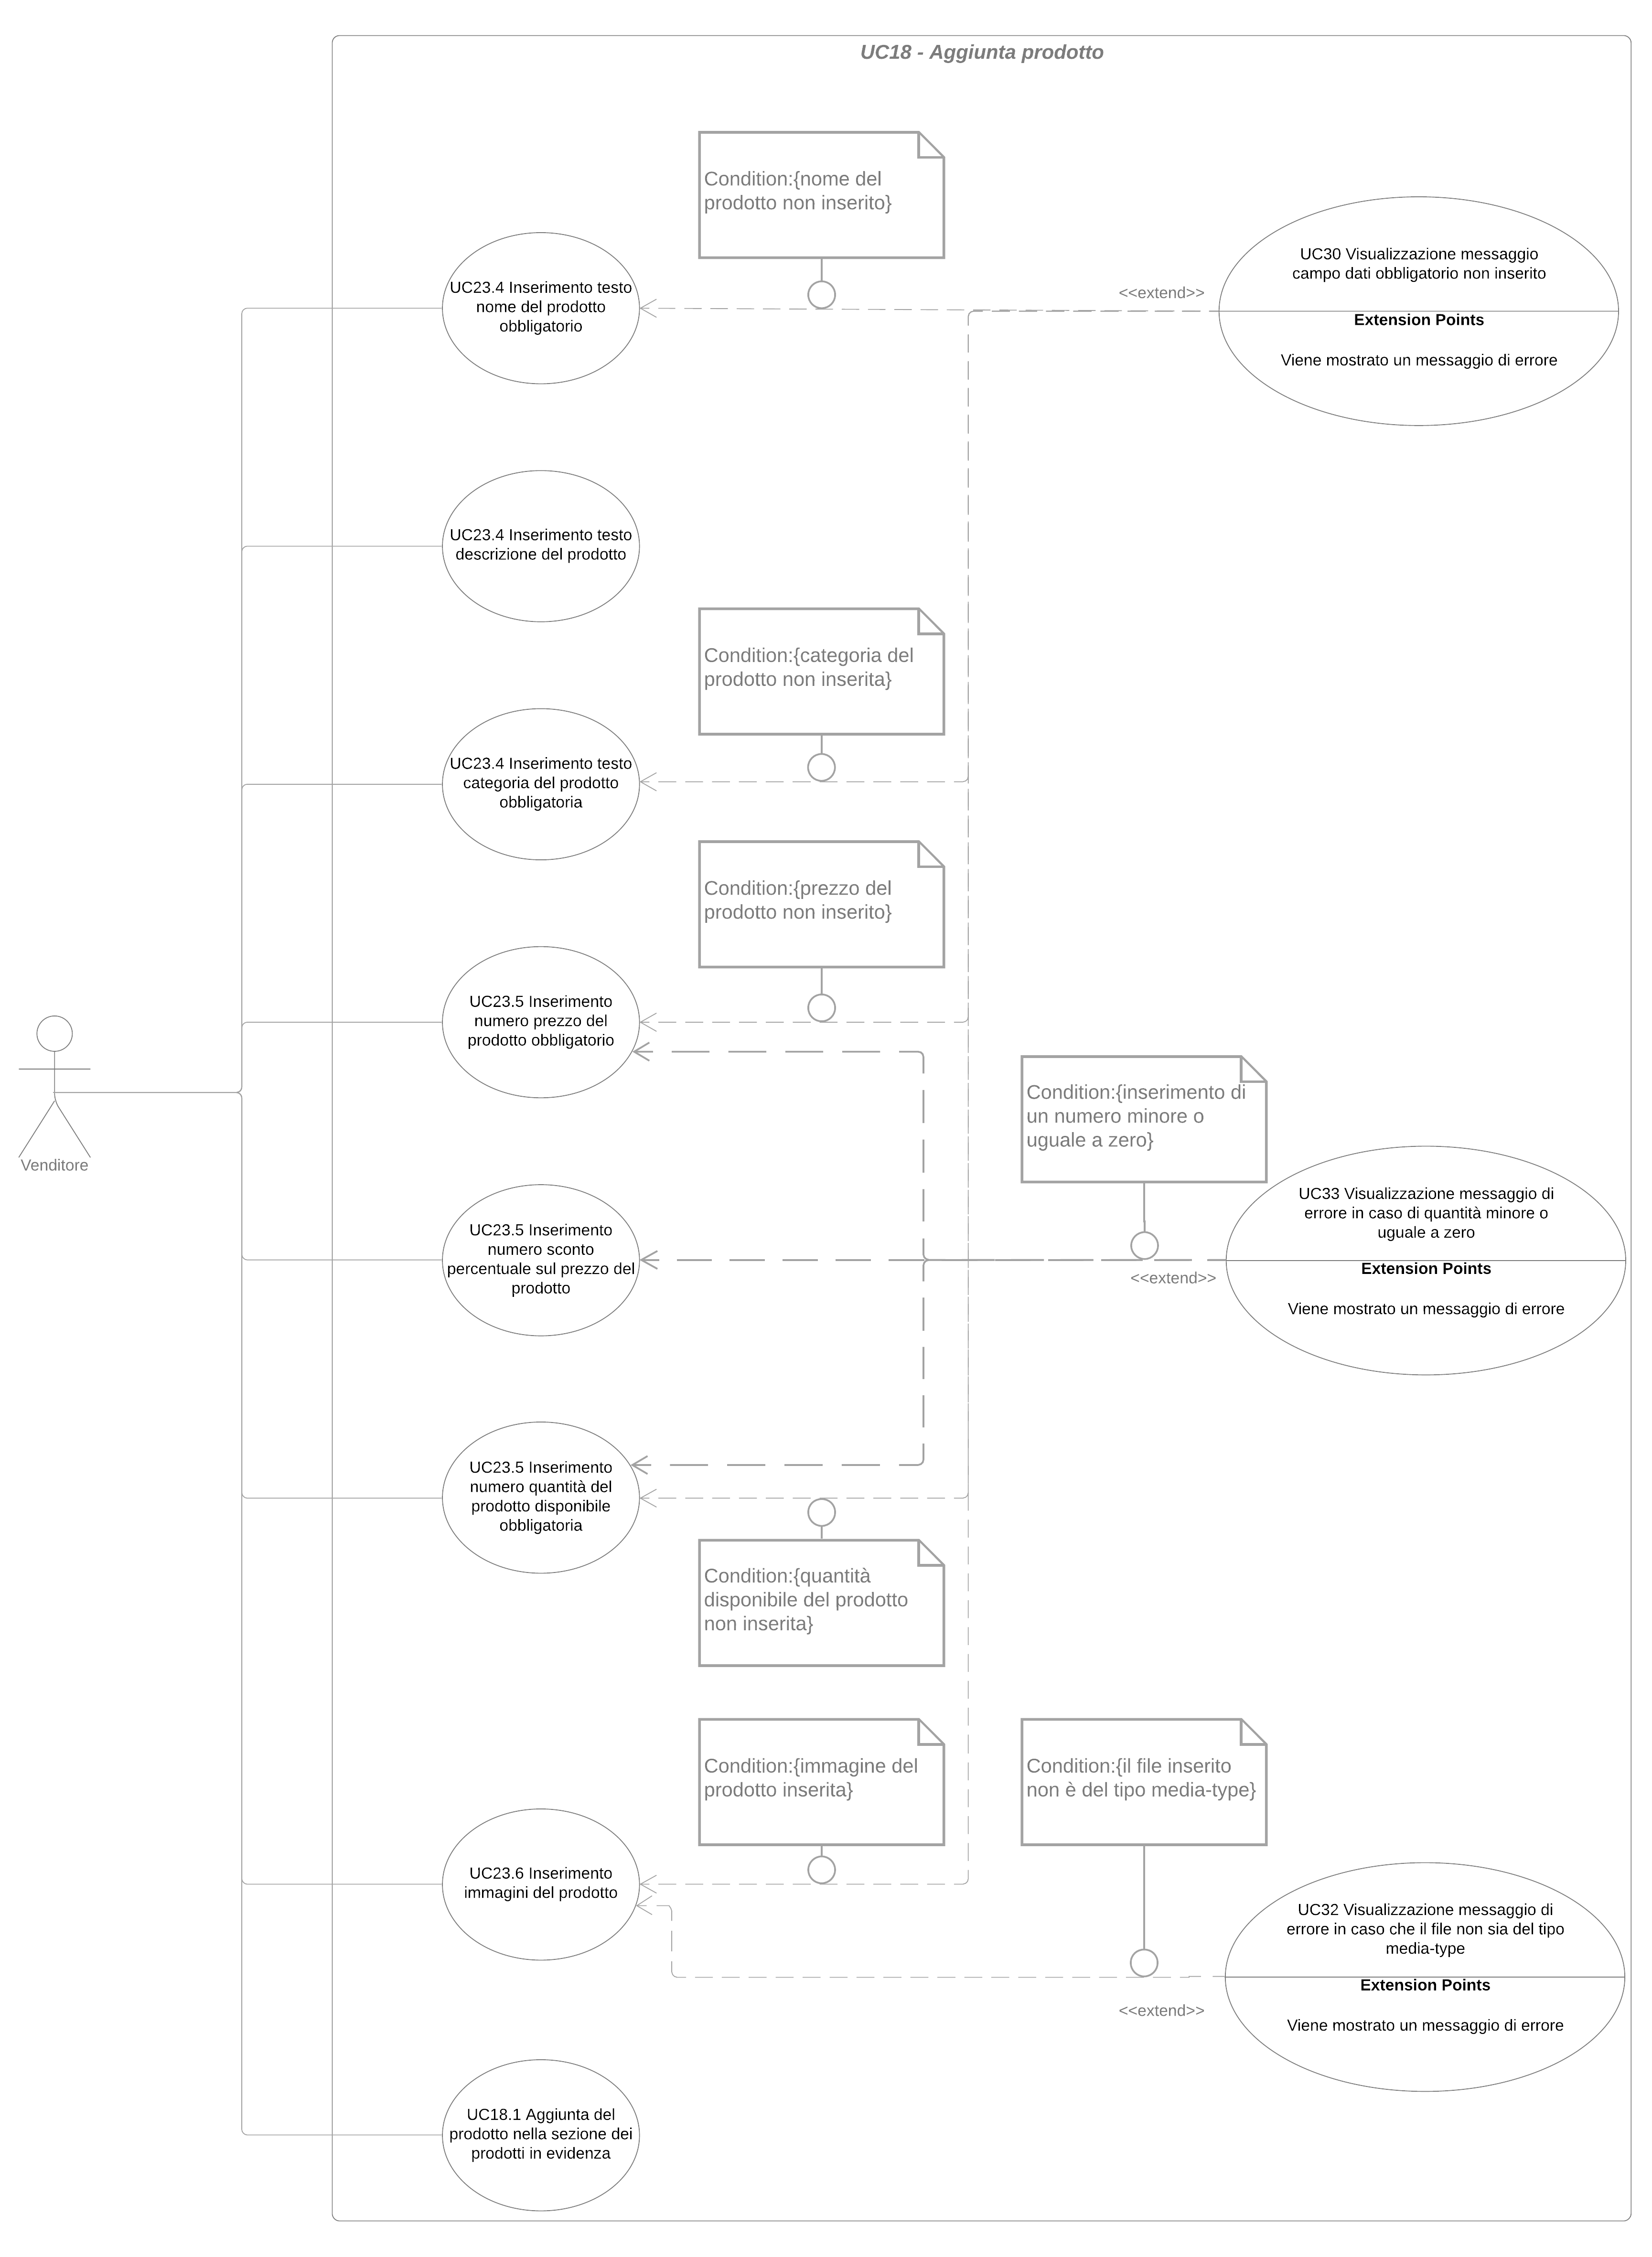
\includegraphics[scale=0.1]{Immagini/DiagrammiUC/UC18AggiuntaProdotto.png}
    \caption{Diagramma di \actualUC: Aggiunta di un prodotto nella piattaforma da parte del venditore} 
    \label{fig:AggiuntaProdotto}
\end{figure}

Il venditore aggiunge un prodotto alla piattaforma, così da poter essere venduto.
\begin{itemize}
    \item \textbf{Attori Primari:} Venditore.
    \item \textbf{Precondizione:} Il venditore si trova nella pagina della \glo{dashboard} e seleziona l'azione per aggiungere un prodotto.
    \item \textbf{Postcondizione:} Il venditore ha aggiunto il prodotto nella piattaforma.
    \item \textbf{Scenario Principale:} Il venditore preme sull'azione che porta alla pagina di aggiunta di un prodotto e compie i seguenti passi:
    \begin{itemize}
        \item (\actualUC.1) - Inserisce il nome del prodotto obbligatorio.
        \item (\actualUC.2) - Inserisce la descrizione del prodotto.
        \item (\actualUC.3) - Inserisce almeno una categoria del prodotto.
        \item (\actualUC.4) - Inserisce il prezzo del prodotto obbligatorio.
        \item (\actualUC.5) - Inserisce lo sconto percentuale sul prezzo del prodotto.
        \item (\actualUC.6) - Inserisce la quantità del prodotto disponibile obbligatoria.
        \item (\actualUC.7) - Inserisce almeno una e al massimo quattro foto del prodotto.
        \item (\actualUC.8) - Seleziona se il prodotto è da inserire tra quelli in evidenza.
        \item Conferma gli inserimenti e aggiunge il prodotto alla piattaforma.
    \end{itemize}
    \item \textbf{Estensioni:}
    \begin{itemize}
        \item (UC30) - Visualizzazione messaggio nome del prodotto non inserito.
        \item (UC30) - Visualizzazione messaggio categoria del prodotto non inserita.
        \item (UC30) - Visualizzazione messaggio prezzo del prodotto non inserito.
        \item (UC30) - Visualizzazione messaggio quantità del prodotto non inserita.
        \item (UC30) - Visualizzazione messaggio foto del prodotto non inserita.
    \end{itemize}
\end{itemize}

\resetSubUC

\subUC{Inserimento del nome obbligatorio}


\begin{itemize}
    \item \textbf{Attori Primari:} Venditore.
    \item \textbf{Precondizione:} Il venditore si trova nella pagina della \glo{dashboard} e seleziona l'azione per aggiungere un prodotto.
    \item \textbf{Postcondizione:} Il venditore ha aggiunto il prodotto nella piattaforma.
    \item \textbf{Scenario Principale:} Il venditore preme sull'azione che porta alla pagina di aggiunta di un prodotto e compie i seguenti passi:
    \item \textbf{Estensioni:}
    \begin{itemize}
        \item (UC30) - Visualizzazione messaggio nome del prodotto non inserito.
        \item (UC30) - Visualizzazione messaggio categoria del prodotto non inserita.
        \item (UC30) - Visualizzazione messaggio prezzo del prodotto non inserito.
        \item (UC30) - Visualizzazione messaggio quantità del prodotto non inserita.
        \item (UC30) - Visualizzazione messaggio foto del prodotto non inserita.
    \end{itemize}
\end{itemize}


\UC{Aggiunta o rimozione prodotto nella sezione dei prodotti in evidenza}
Il venditore aggiunge o rimuove un prodotto nella sezione dei prodotti in evidenza presente nella home.
\begin{itemize}
    \item \textbf{Attori Primari:} Venditore.
    \item \textbf{Precondizione:} Il venditore si trova nella pagina di aggiunta o modifica di un prodotto e ha premuto sull'azione di aggiunta o rimozione del prodotto nella sezione dei prodotti in evidenza.
    \item \textbf{Postcondizione:} Il prodotto viene aggiunto o rimosso, in base al suo stato attuale, nella sezione sezione dei prodotti in evidenza. 
    \item \textbf{Scenario Principale:} Il venditore vuole aggiungere o rimuovere un prodotto nella sezione dei prodotti in evidenza presente nella home e clicca sulla rispettiva azione.
\end{itemize}

\UC{Modifica prodotto}

\begin{figure}[H]
    \centering
    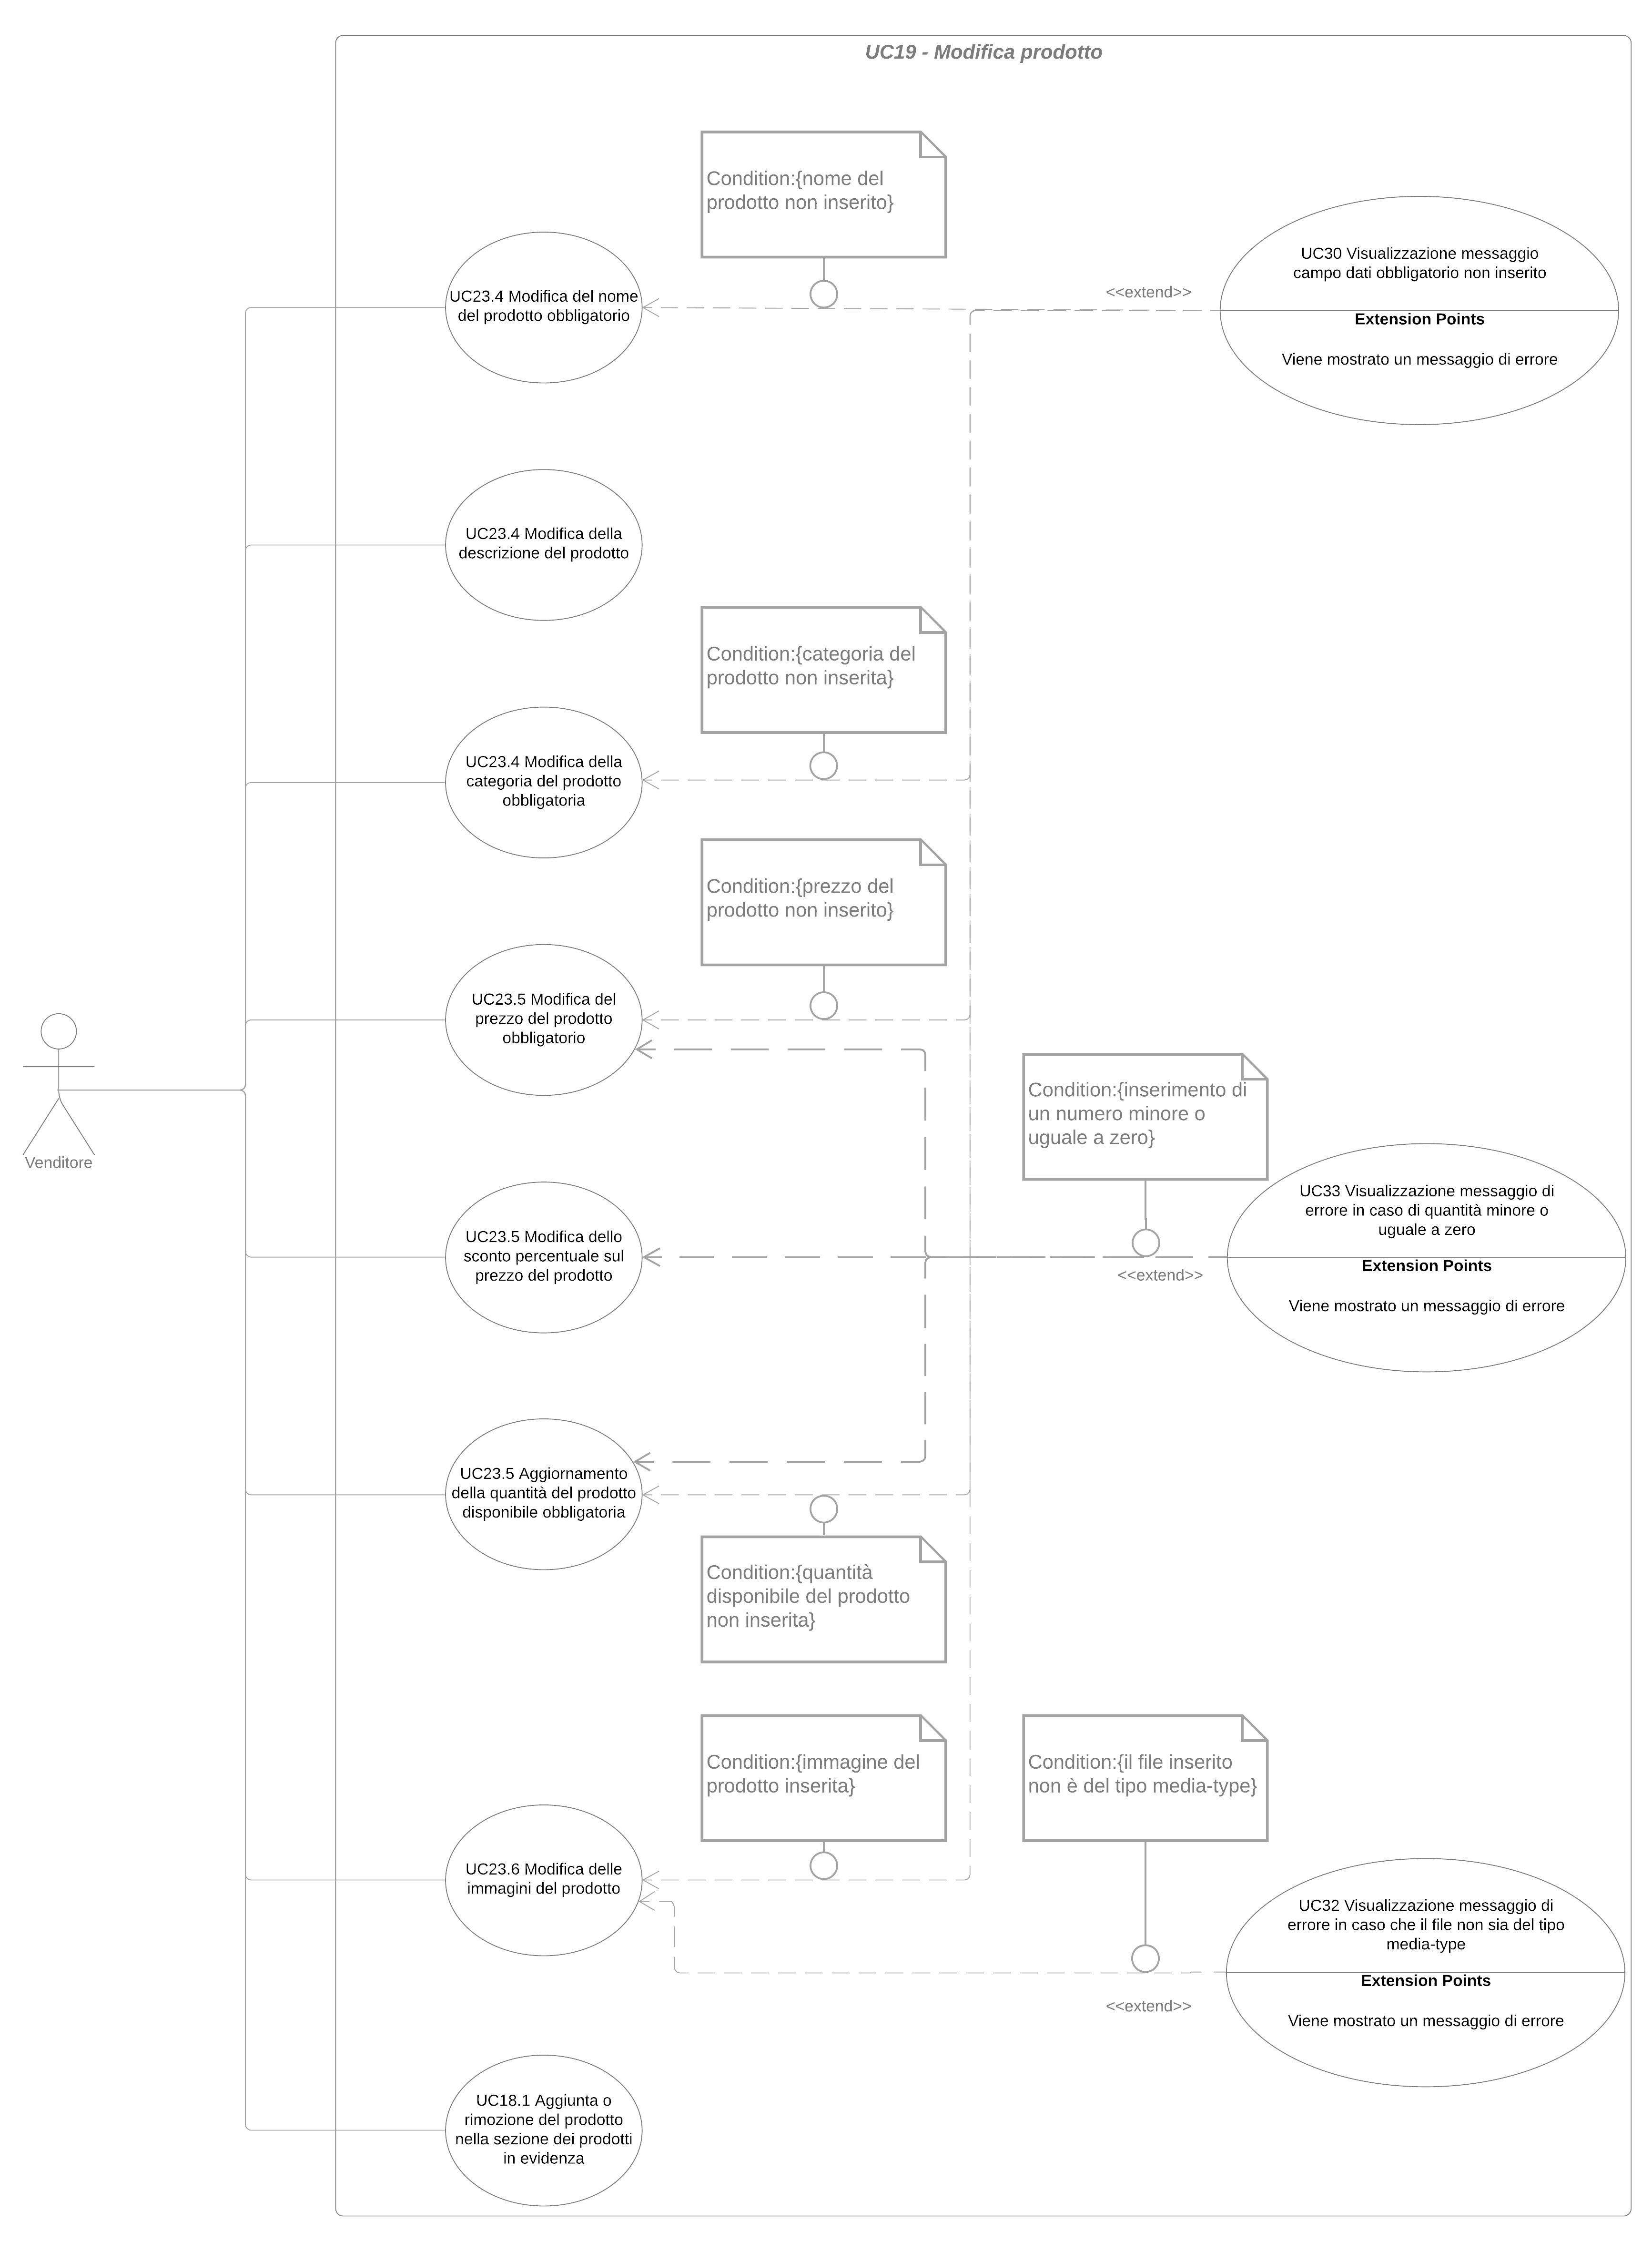
\includegraphics[scale=0.1]{Immagini/DiagrammiUC/UC19ModificaProdotto.png}
    \caption{Diagramma di \actualUC: Modifica di un prodotto nella piattaforma da parte del venditore}
    \label{fig:ModificaProdotto}
\end{figure}

Il venditore modifica uno o più campi di un prodotto della piattaforma.
\begin{itemize}
    \item \textbf{Attori Primari:} Venditore.
    \item \textbf{Precondizione:} Il venditore si trova nella pagina della dashboard e seleziona un prodotto già presente.
    \item \textbf{Postcondizione:} Il venditore ha modificato il prodotto con le modifiche selezionato.
    \item \textbf{Scenario Principale:} Il venditore preme sull'azione che porta alla pagina di modifica di un prodotto e compie zero, o più, dei seguenti passi:
    \begin{itemize}
        \item (UC23.4) - Inserisce il nuovo nome del prodotto obbligatorio.
        \item (UC23.4) - Inserisce la nuova descrizione del prodotto.
        \item (UC23.4) - Inserisce le nuove categorie del prodotto.
        \item (UC23.5) - Inserisce il nuovo prezzo del prodotto obbligatorio.
        \item (UC23.5) - Inserisce il nuovo sconto percentuale sul prezzo del prodotto.
        \item (UC23.5) - Inserisce la nuova quantità del prodotto disponibile obbligatoria.
        \item (UC23.6) - Aggiunge o rimuove le foto del prodotto, sempre lasciandone almeno una.
        \item (UC18.1) - Aggiunge o rimuove il prodotto, in base al suo stato attuale, nella sezione dei prodotti in evidenza presente nella home.
        \item conferma gli inserimenti e il prodotto viene modificato.
    \end{itemize}
    \item \textbf{Estensioni:}
    \begin{itemize}
        \item (UC30) - Visualizzazione messaggio nome del prodotto non inserito.
        \item (UC30) - Visualizzazione messaggio categoria del prodotto non inserita.
        \item (UC30) - Visualizzazione messaggio prezzo del prodotto non inserito.
        \item (UC30) - Visualizzazione messaggio quantità del prodotto non inserita.
        \item (UC30) - Visualizzazione messaggio foto del prodotto non inserita.
    \end{itemize}
\end{itemize}

\UC{Eliminazione prodotto}
\begin{figure}[H]
    \centering
    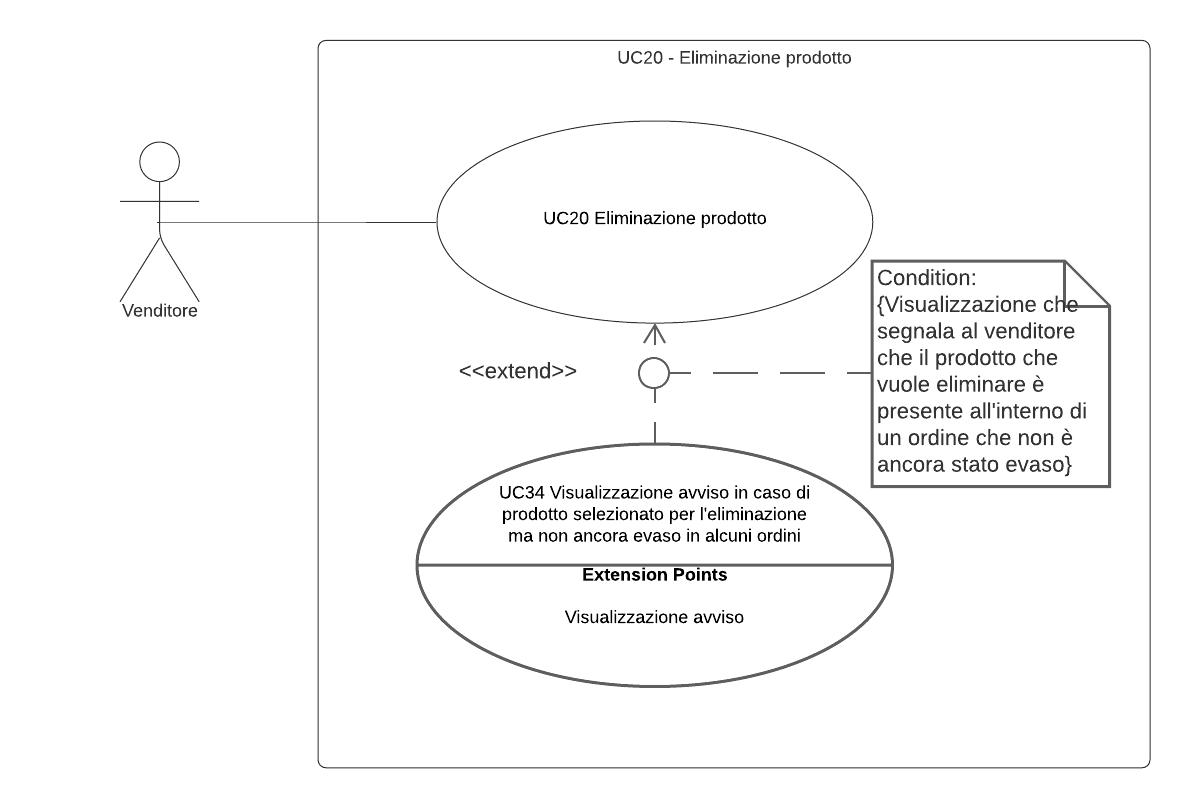
\includegraphics[width=\textwidth]{Immagini/DiagrammiUC/UC20EliminazioneProdotto}
    \caption{Diagramma di \actualUC: Eliminazione di un prodotto da parte del venditore} 
    \label{fig:EliminazioneProdotto}
\end{figure}

Il venditore vuole eliminare un prodotto precedentemente inserito.
\begin{itemize}
    \item \textbf{Attori Primari:} Venditore.
    \item \textbf{Precondizione:} Il venditore si trova nella pagina della dashboard.
    \item \textbf{Postcondizione:} Il venditore ha eliminato il prodotto selezionato.
    \item \textbf{Scenario Principale:} Il venditore seleziona un prodotto dalla lista di quelli che ha inserito nella piattaforma e preme sul link per eliminarlo definitivamente.
    \begin{itemize}
    \item Il prodotto viene rimosso da PDP, PLP, home, carrelli e dashboard.
    \item Il prodotto rimane negli ordini già effettuati.
    \end{itemize}
    \item \textbf{Scenario Alternativo:} Il venditore seleziona per l'eliminazione, un prodotto che è stato ordinato ma non ancora pagato quindi verrà visualizzato un messaggio di errore e viene negata la possibilità di eliminare il prodotto selezionato.
    \item \textbf{Estensioni:}
    \begin{itemize}
        \item (UC34) - Visualizzazione avviso in caso di prodotto selezionato per l’eliminazione ma non ancora evaso in alcuni ordini.
    \end{itemize}
\end{itemize}

\UC{Rifornimento prodotto}
Il venditore vuole rifornire un prodotto precedentemente inserito che sta per esaurire o è esaurito.
\begin{itemize}
    \item \textbf{Attori Primari:} Venditore.
    \item \textbf{Precondizione:} Il venditore si trova nella pagina della dashboard.
    \item \textbf{Postcondizione:} Il venditore ha rifornito un prodotto.
    \item \textbf{Scenario Principale:} Il venditore seleziona un prodotto dalla lista di quelli che ha inserito nella piattaforma e preme sull'azione per rifornirlo. Per completare il rifornimento deve svolgere i seguenti passi:
    \begin{itemize}
        \item (UC23.5) - Inserisce la quantità.
        \item Preme sull'azione per il salvataggio della modifica.
    \end{itemize}
\end{itemize}

\UC{Lista riepilogo ordini}
Il venditore visualizza una lista con tutti gli ordini effettuati.
\begin{itemize}
    \item \textbf{Attori Primari:} Venditore.
    \item \textbf{Precondizione:} Il venditore accede alla dashboard.
    \item \textbf{Postcondizione:} Viene visualizzata una lista con tutti gli ordini effettuati non ancora evasi, specificandone anche l'email del richiedente.
    \item \textbf{Scenario Principale:} Il venditore accede alla dashboard e visualizza gli ordini effettuati dagli acquirenti che non sono ancora stati evasi. Le azioni che il venditore potrà compiere dalla lista sono: 
    \begin{itemize}
        \item Visualizzare solo i prodotti non evasi (opzione di default), visualizzare solo gli ordini evasi o visualizzarli entrambi.
        \item Evadere un ordine.
        \item Accedere alla pagina di riepilogo ordine premendo sull'azione opportuna (UC14).
    \end{itemize}
\end{itemize}
